% Created by tikzDevice version 0.10.1 on 2016-08-29 22:50:27
% !TEX encoding = UTF-8 Unicode
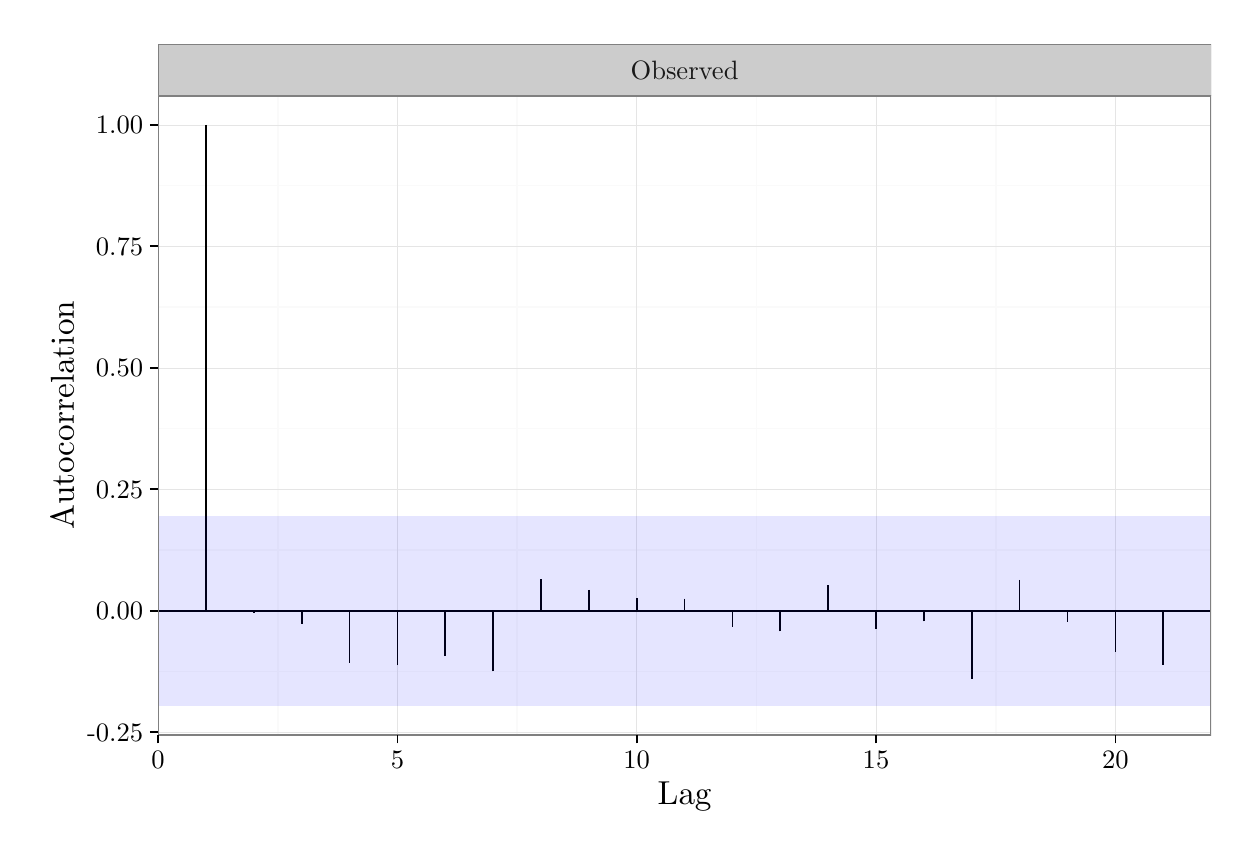
\begin{tikzpicture}[x=1pt,y=1pt]
\definecolor{fillColor}{RGB}{255,255,255}
\path[use as bounding box,fill=fillColor,fill opacity=0.00] (0,0) rectangle (433.62,289.08);
\begin{scope}
\path[clip] (  0.00,  0.00) rectangle (433.62,289.08);
\definecolor{drawColor}{RGB}{255,255,255}
\definecolor{fillColor}{RGB}{255,255,255}

\path[draw=drawColor,line width= 0.6pt,line join=round,line cap=round,fill=fillColor] (  0.00,  0.00) rectangle (433.62,289.08);
\end{scope}
\begin{scope}
\path[clip] ( 47.13, 33.48) rectangle (427.62,264.47);
\definecolor{fillColor}{RGB}{255,255,255}

\path[fill=fillColor] ( 47.13, 33.48) rectangle (427.62,264.47);
\definecolor{drawColor}{gray}{0.98}

\path[draw=drawColor,line width= 0.6pt,line join=round] ( 47.13, 56.44) --
	(427.62, 56.44);

\path[draw=drawColor,line width= 0.6pt,line join=round] ( 47.13,100.34) --
	(427.62,100.34);

\path[draw=drawColor,line width= 0.6pt,line join=round] ( 47.13,144.23) --
	(427.62,144.23);

\path[draw=drawColor,line width= 0.6pt,line join=round] ( 47.13,188.13) --
	(427.62,188.13);

\path[draw=drawColor,line width= 0.6pt,line join=round] ( 47.13,232.02) --
	(427.62,232.02);

\path[draw=drawColor,line width= 0.6pt,line join=round] ( 90.36, 33.48) --
	( 90.36,264.47);

\path[draw=drawColor,line width= 0.6pt,line join=round] (176.84, 33.48) --
	(176.84,264.47);

\path[draw=drawColor,line width= 0.6pt,line join=round] (263.32, 33.48) --
	(263.32,264.47);

\path[draw=drawColor,line width= 0.6pt,line join=round] (349.79, 33.48) --
	(349.79,264.47);
\definecolor{drawColor}{gray}{0.90}

\path[draw=drawColor,line width= 0.2pt,line join=round] ( 47.13, 34.49) --
	(427.62, 34.49);

\path[draw=drawColor,line width= 0.2pt,line join=round] ( 47.13, 78.39) --
	(427.62, 78.39);

\path[draw=drawColor,line width= 0.2pt,line join=round] ( 47.13,122.28) --
	(427.62,122.28);

\path[draw=drawColor,line width= 0.2pt,line join=round] ( 47.13,166.18) --
	(427.62,166.18);

\path[draw=drawColor,line width= 0.2pt,line join=round] ( 47.13,210.07) --
	(427.62,210.07);

\path[draw=drawColor,line width= 0.2pt,line join=round] ( 47.13,253.97) --
	(427.62,253.97);

\path[draw=drawColor,line width= 0.2pt,line join=round] ( 47.13, 33.48) --
	( 47.13,264.47);

\path[draw=drawColor,line width= 0.2pt,line join=round] (133.60, 33.48) --
	(133.60,264.47);

\path[draw=drawColor,line width= 0.2pt,line join=round] (220.08, 33.48) --
	(220.08,264.47);

\path[draw=drawColor,line width= 0.2pt,line join=round] (306.55, 33.48) --
	(306.55,264.47);

\path[draw=drawColor,line width= 0.2pt,line join=round] (393.03, 33.48) --
	(393.03,264.47);
\definecolor{drawColor}{RGB}{0,0,0}

\path[draw=drawColor,line width= 0.6pt,line join=round] ( 47.13, 78.39) -- (427.62, 78.39);

\path[draw=drawColor,line width= 0.6pt,line join=round] ( 64.42,253.97) -- ( 64.42, 78.39);

\path[draw=drawColor,line width= 0.6pt,line join=round] ( 81.72, 77.75) -- ( 81.72, 78.39);

\path[draw=drawColor,line width= 0.6pt,line join=round] ( 99.01, 73.64) -- ( 99.01, 78.39);

\path[draw=drawColor,line width= 0.6pt,line join=round] (116.31, 59.54) -- (116.31, 78.39);

\path[draw=drawColor,line width= 0.6pt,line join=round] (133.60, 58.62) -- (133.60, 78.39);

\path[draw=drawColor,line width= 0.6pt,line join=round] (150.90, 61.99) -- (150.90, 78.39);

\path[draw=drawColor,line width= 0.6pt,line join=round] (168.19, 56.49) -- (168.19, 78.39);

\path[draw=drawColor,line width= 0.6pt,line join=round] (185.49, 89.80) -- (185.49, 78.39);

\path[draw=drawColor,line width= 0.6pt,line join=round] (202.78, 85.95) -- (202.78, 78.39);

\path[draw=drawColor,line width= 0.6pt,line join=round] (220.08, 82.95) -- (220.08, 78.39);

\path[draw=drawColor,line width= 0.6pt,line join=round] (237.37, 82.72) -- (237.37, 78.39);

\path[draw=drawColor,line width= 0.6pt,line join=round] (254.67, 72.68) -- (254.67, 78.39);

\path[draw=drawColor,line width= 0.6pt,line join=round] (271.96, 70.95) -- (271.96, 78.39);

\path[draw=drawColor,line width= 0.6pt,line join=round] (289.26, 87.66) -- (289.26, 78.39);

\path[draw=drawColor,line width= 0.6pt,line join=round] (306.55, 71.76) -- (306.55, 78.39);

\path[draw=drawColor,line width= 0.6pt,line join=round] (323.85, 74.51) -- (323.85, 78.39);

\path[draw=drawColor,line width= 0.6pt,line join=round] (341.14, 53.77) -- (341.14, 78.39);

\path[draw=drawColor,line width= 0.6pt,line join=round] (358.44, 89.51) -- (358.44, 78.39);

\path[draw=drawColor,line width= 0.6pt,line join=round] (375.73, 74.36) -- (375.73, 78.39);

\path[draw=drawColor,line width= 0.6pt,line join=round] (393.03, 63.60) -- (393.03, 78.39);

\path[draw=drawColor,line width= 0.6pt,line join=round] (410.32, 58.80) -- (410.32, 78.39);
\definecolor{fillColor}{RGB}{0,0,255}

\path[fill=fillColor,fill opacity=0.10] ( 47.13, 43.98) rectangle (427.62,112.80);
\definecolor{drawColor}{gray}{0.50}

\path[draw=drawColor,line width= 0.6pt,line join=round,line cap=round] ( 47.13, 33.48) rectangle (427.62,264.47);
\end{scope}
\begin{scope}
\path[clip] ( 47.13,264.47) rectangle (427.62,283.08);
\definecolor{drawColor}{gray}{0.50}
\definecolor{fillColor}{gray}{0.80}

\path[draw=drawColor,line width= 0.2pt,line join=round,line cap=round,fill=fillColor] ( 47.13,264.47) rectangle (427.62,283.08);
\definecolor{drawColor}{gray}{0.10}

\node[text=drawColor,anchor=base,inner sep=0pt, outer sep=0pt, scale=  0.96] at (237.37,270.47) {Observed};
\end{scope}
\begin{scope}
\path[clip] (  0.00,  0.00) rectangle (433.62,289.08);
\definecolor{drawColor}{RGB}{0,0,0}

\node[text=drawColor,anchor=base east,inner sep=0pt, outer sep=0pt, scale=  0.96] at ( 41.73, 31.19) {-0.25};

\node[text=drawColor,anchor=base east,inner sep=0pt, outer sep=0pt, scale=  0.96] at ( 41.73, 75.08) {0.00};

\node[text=drawColor,anchor=base east,inner sep=0pt, outer sep=0pt, scale=  0.96] at ( 41.73,118.98) {0.25};

\node[text=drawColor,anchor=base east,inner sep=0pt, outer sep=0pt, scale=  0.96] at ( 41.73,162.87) {0.50};

\node[text=drawColor,anchor=base east,inner sep=0pt, outer sep=0pt, scale=  0.96] at ( 41.73,206.77) {0.75};

\node[text=drawColor,anchor=base east,inner sep=0pt, outer sep=0pt, scale=  0.96] at ( 41.73,250.66) {1.00};
\end{scope}
\begin{scope}
\path[clip] (  0.00,  0.00) rectangle (433.62,289.08);
\definecolor{drawColor}{RGB}{0,0,0}

\path[draw=drawColor,line width= 0.6pt,line join=round] ( 44.13, 34.49) --
	( 47.13, 34.49);

\path[draw=drawColor,line width= 0.6pt,line join=round] ( 44.13, 78.39) --
	( 47.13, 78.39);

\path[draw=drawColor,line width= 0.6pt,line join=round] ( 44.13,122.28) --
	( 47.13,122.28);

\path[draw=drawColor,line width= 0.6pt,line join=round] ( 44.13,166.18) --
	( 47.13,166.18);

\path[draw=drawColor,line width= 0.6pt,line join=round] ( 44.13,210.07) --
	( 47.13,210.07);

\path[draw=drawColor,line width= 0.6pt,line join=round] ( 44.13,253.97) --
	( 47.13,253.97);
\end{scope}
\begin{scope}
\path[clip] (  0.00,  0.00) rectangle (433.62,289.08);
\definecolor{drawColor}{RGB}{0,0,0}

\path[draw=drawColor,line width= 0.6pt,line join=round] ( 47.13, 30.48) --
	( 47.13, 33.48);

\path[draw=drawColor,line width= 0.6pt,line join=round] (133.60, 30.48) --
	(133.60, 33.48);

\path[draw=drawColor,line width= 0.6pt,line join=round] (220.08, 30.48) --
	(220.08, 33.48);

\path[draw=drawColor,line width= 0.6pt,line join=round] (306.55, 30.48) --
	(306.55, 33.48);

\path[draw=drawColor,line width= 0.6pt,line join=round] (393.03, 30.48) --
	(393.03, 33.48);
\end{scope}
\begin{scope}
\path[clip] (  0.00,  0.00) rectangle (433.62,289.08);
\definecolor{drawColor}{RGB}{0,0,0}

\node[text=drawColor,anchor=base,inner sep=0pt, outer sep=0pt, scale=  0.96] at ( 47.13, 21.46) {0};

\node[text=drawColor,anchor=base,inner sep=0pt, outer sep=0pt, scale=  0.96] at (133.60, 21.46) {5};

\node[text=drawColor,anchor=base,inner sep=0pt, outer sep=0pt, scale=  0.96] at (220.08, 21.46) {10};

\node[text=drawColor,anchor=base,inner sep=0pt, outer sep=0pt, scale=  0.96] at (306.55, 21.46) {15};

\node[text=drawColor,anchor=base,inner sep=0pt, outer sep=0pt, scale=  0.96] at (393.03, 21.46) {20};
\end{scope}
\begin{scope}
\path[clip] (  0.00,  0.00) rectangle (433.62,289.08);
\definecolor{drawColor}{RGB}{0,0,0}

\node[text=drawColor,anchor=base,inner sep=0pt, outer sep=0pt, scale=  1.20] at (237.37,  8.40) {Lag};
\end{scope}
\begin{scope}
\path[clip] (  0.00,  0.00) rectangle (433.62,289.08);
\definecolor{drawColor}{RGB}{0,0,0}

\node[text=drawColor,rotate= 90.00,anchor=base,inner sep=0pt, outer sep=0pt, scale=  1.20] at ( 16.66,148.97) {Autocorrelation};
\end{scope}
\end{tikzpicture}
